\documentclass{standalone}
\usepackage{tikz}
\begin{document}
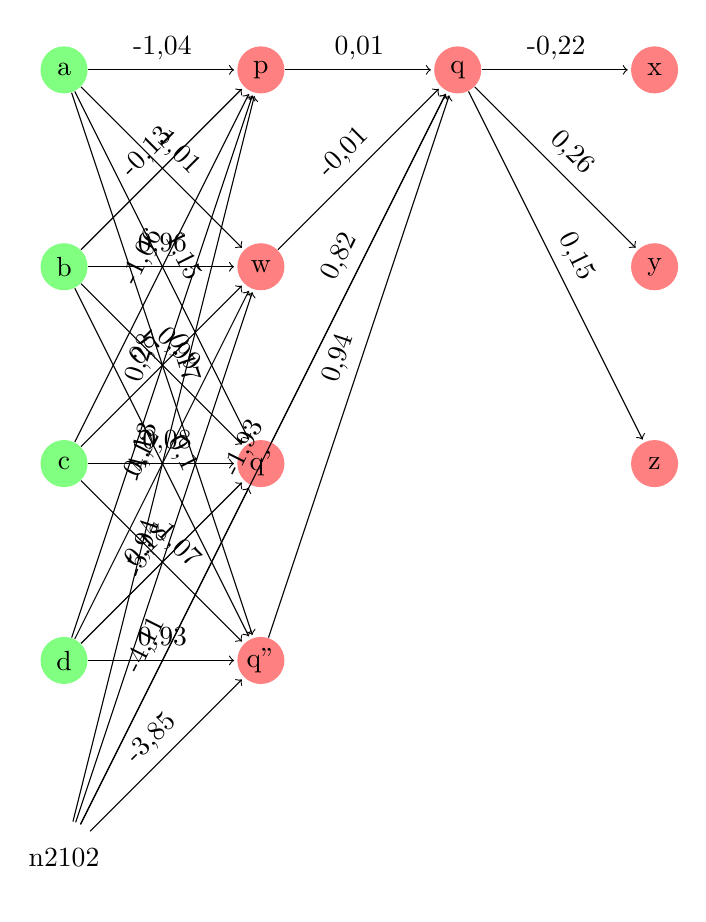
\begin{tikzpicture}[shorten >=1pt,->,draw=black!,node distance=2.5cm]
\tikzstyle{neuron}=[circle,fill=black!25,minimum size=17pt,inner sep=0pt]
\tikzstyle{constant}=[neuron, fill=white!50];
\tikzstyle{sigmoid}=[neuron, fill=red!50];
\tikzstyle{identity}=[neuron, fill=green!50];
\node [identity] (a) {a};
\node [identity,below of=a] (b) {b};
\node [identity,below of=b] (c) {c};
\node [identity,below of=c] (d) {d};
\node [constant,below of=d] (n2102) {n2102};
\node [sigmoid,right of=a] (p) {p};
\node [sigmoid,below of=p] (w) {w};
\node [sigmoid,below of=w] (q') {q'};
\node [sigmoid,below of=q'] (q'') {q''};
\node [sigmoid,right of=p] (q) {q};
\node [sigmoid,right of=q] (x) {x};
\node [sigmoid,below of=x] (y) {y};
\node [sigmoid,below of=y] (z) {z};
\path[every node/.style={sloped,anchor=south,auto=false}]
(w) edge node {-0,01} (q)
(p) edge node {0,01} (q)
(q'') edge node {0,94} (q)
(q') edge node {0,82} (q)
(q) edge node {0,26} (y)
(q) edge node {-0,22} (x)
(q) edge node {0,15} (z)
(b) edge node {0,1} (q'')
(b) edge node {0,99} (q')
(b) edge node {0,96} (w)
(b) edge node {-0,13} (p)
(a) edge node {1,15} (q')
(a) edge node {1,01} (w)
(a) edge node {0,17} (q'')
(a) edge node {-1,04} (p)
(d) edge node {0,12} (w)
(d) edge node {0,28} (p)
(d) edge node {0,93} (q'')
(d) edge node {0,18} (q')
(c) edge node {1,07} (q'')
(c) edge node {-1,06} (p)
(c) edge node {-0,08} (q')
(c) edge node {0,7} (w)
(n2102) edge node {-1,93} (q)
(n2102) edge node {-4,11} (q')
(n2102) edge node {-3,85} (q'')
(n2102) edge node {-4,13} (p)
(n2102) edge node {-5,94} (w)
;\end{tikzpicture}
\end{document}